\documentclass[14pt]{extarticle}
\def\activityid{F10-K-v3}\usepackage[letterpaper,margin=.65in,top=.60in,bottom=.65in]{geometry}
\usepackage[T1]{fontenc}
\usepackage[default]{sourcesanspro}
\usepackage{microtype,tikz,array,tabularx,fancyhdr,amsmath,amssymb}
\usepackage[hidelinks]{hyperref}
\usetikzlibrary{calc,arrows.meta}
\setlength{\parindent}{0pt}\setlength{\parskip}{7pt}
\setlength{\headheight}{0pt}\setlength{\footskip}{26pt}\setlength{\emergencystretch}{2em}
\pagestyle{fancy}\fancyhf{}\renewcommand{\headrulewidth}{0pt}\renewcommand{\footrulewidth}{.4pt}
\fancyfoot[L]{\scriptsize Bellingham Math Circle / Week 10 / \activityid}
\fancyfoot[R]{\scriptsize \thepage}
\definecolor{ink}{gray}{.12}\definecolor{soft}{gray}{.95}\color{ink}
\newcommand{\PageTitle}[2]{{\fontsize{10}{12}\selectfont\bfseries WEEK 10\quad ROUTE LAB\hfill #1\par}\vspace{3pt}{\fontsize{26}{29}\selectfont\bfseries #2\par}\vspace{2pt}}
\newcommand{\Subhead}[1]{\par\vspace{3pt}{\large\bfseries #1}\par}
\newcommand{\RuleBox}[1]{\par\begingroup\setlength{\fboxsep}{8pt}\colorbox{soft}{\parbox{\dimexpr\linewidth-16pt\relax}{#1}}\endgroup\par}
\newcommand{\WriteBox}[2]{\par\textbf{#1}\par\vspace{2pt}\begin{tikzpicture}\draw[black!40,line width=.5pt] (0,0) rectangle (\dimexpr\linewidth-.5pt\relax,#2);\end{tikzpicture}\par}
\newcommand{\RookBoard}[3]{\begin{tikzpicture}[x=#3,y=#3]\draw[step=1,black!45] (0,0) grid (#1,#2);\draw[thick] (0,0) rectangle (#1,#2);\node[font=\Large] at ({#1-.5},.5){$\star$};\draw[-{Latex},thick] (0,-.35)--(#1,-.35);\draw[-{Latex},thick] ({#1+.35},#2)--({#1+.35},0);\end{tikzpicture}}
\newcommand{\Table}[3]{\begin{tikzpicture}[x=#3,y=#3]\draw[step=1,black!25] (0,0) grid (#1,#2);\draw[thick] (0,0) rectangle (#1,#2);\fill (0,0)circle(3pt);\draw[-{Latex},very thick] (0,0)--(.7,.7);\node[below] at ({#1/2},-.1){width #1};\node[rotate=90,above] at (-.2,{#2/2}){height #2};\end{tikzpicture}}
\newcommand{\GraphNodes}{\coordinate(A)at(0,0);\coordinate(B)at(3,0);\coordinate(C)at(1.5,2.6);\coordinate(D)at(1.5,.95);}
\newcommand{\Kfour}[1]{\begin{tikzpicture}[scale=#1]\GraphNodes\draw[very thick](A)--(B)--(C)--(A)--(D)--(B) (D)--(C);\foreach \n in {A,B,C,D}{\node[circle,draw,fill=white,minimum size=22pt,font=\bfseries]at(\n){\n};}\end{tikzpicture}}
\newcommand{\House}[1]{\begin{tikzpicture}[scale=#1]\coordinate(A)at(0,0);\coordinate(B)at(3,0);\coordinate(C)at(3,2);\coordinate(D)at(0,2);\coordinate(E)at(1.5,3.3);\draw[very thick](A)--(B)--(C)--(D)--(A) (D)--(E)--(C);\foreach \n in {A,B,C,D,E}{\node[circle,draw,fill=white,minimum size=22pt,font=\bfseries]at(\n){\n};}\end{tikzpicture}}




\newcommand{\StudentPage}[1]{{\fontsize{10}{12}\selectfont\bfseries Week 10 / Route lab / #1\par}\vspace{10pt}}
\newcommand{\Problem}[2]{\par\noindent\textbf{Problem #1:} #2\par}
\newcommand{\Space}[1]{\par\begin{tikzpicture}\draw[black!35] (0,0) rectangle (\dimexpr\linewidth-.5pt\relax,#1);\end{tikzpicture}\par}
\newcommand{\Piles}[1]{\begin{center}\begin{tikzpicture}[x=1in,y=1in]\foreach \x in {0,...,#1}{\draw[black!50,rounded corners] ({\x*2.05},0) rectangle ({\x*2.05+1.8},1.3);}\end{tikzpicture}\end{center}}

\newcommand{\Triangle}[1]{\begin{tikzpicture}[scale=#1]\draw[very thick](0,0)--(2,0)--(1,1.7)--cycle;\foreach\n/\x/\y in{A/0/0,B/2/0,C/1/1.7}{\node[circle,draw,fill=white,minimum size=25pt]at(\x,\y){\n};}\end{tikzpicture}}
\newcommand{\Branch}[1]{\begin{tikzpicture}[scale=#1]\draw[very thick](0,0)--(2,0)--(1,1.7)--cycle (0,0)--(-1.2,-.8);\foreach\n/\x/\y in{A/0/0,B/2/0,C/1/1.7,D/-1.2/-.8}{\node[circle,draw,fill=white,minimum size=25pt]at(\x,\y){\n};}\end{tikzpicture}}
\newcommand{\StarGraph}[1]{\begin{tikzpicture}[scale=#1]\draw[very thick](0,0)--(0,1.5) (0,0)--(-1.5,-1) (0,0)--(1.5,-1);\foreach\n/\x/\y in{A/0/0,B/0/1.5,C/-1.5/-1,D/1.5/-1}{\node[circle,draw,fill=white,minimum size=25pt]at(\x,\y){\n};}\end{tikzpicture}}
\newcommand{\TwoLoops}[1]{\begin{tikzpicture}[scale=#1]\coordinate(A)at(0,0);\coordinate(B)at(-1.5,1.25);\coordinate(C)at(-1.5,-1.25);\coordinate(D)at(1.5,1.25);\coordinate(E)at(1.5,-1.25);\draw[very thick](A)--(B)--(C)--(A)--(D)--(E)--(A);\foreach\n in{A,B,C,D,E}{\node[circle,draw,fill=white,minimum size=22pt]at(\n){\n};}\end{tikzpicture}}
\newcommand{\WeightedGraph}[1]{\begin{tikzpicture}[scale=#1]\GraphNodes\draw[very thick](A)--node[midway,fill=white,inner sep=1.5pt]{2}(B)--node[midway,fill=white,inner sep=1.5pt]{3}(C)--node[midway,fill=white,inner sep=1.5pt]{7}(A);\draw[very thick](A)--node[midway,fill=white,inner sep=1.5pt]{1}(D)--node[midway,fill=white,inner sep=1.5pt]{6}(B) (D)--node[midway,fill=white,inner sep=1.5pt]{1}(C);\foreach\n in{A,B,C,D}{\node[circle,draw,fill=white,minimum size=22pt,font=\bfseries]at(\n){\n};}\end{tikzpicture}}

\begin{document}

\StudentPage{K--1}
\Problem{1}{Dots are islands; lines are bridges. Move a counter along every bridge once without jumping. You may visit an island again. Mark a bridge after you use it. Try this town from A, then from B. Draw arrows for one complete walk.}
\begin{center}\Triangle{2.8}\end{center}
\Problem{2}{This town has one extra bridge. Try a walk from D, then try from B. Mark used bridges as you go. Circle a place where you can start a walk using every bridge once.}
\begin{center}\Branch{2.3}\end{center}
\newpage
\StudentPage{K--1}
\Problem{3}{Try a walk using every bridge once in each town. Mark used bridges. Circle where a complete walk starts and ends. If you get stuck, reset and try a different start.}
\begin{center}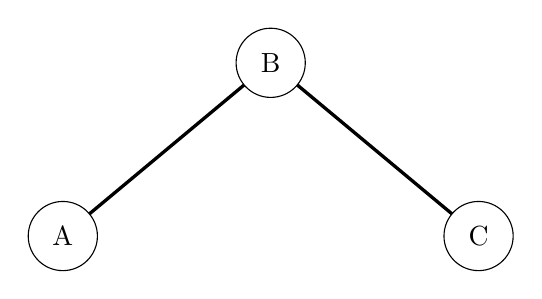
\begin{tikzpicture}[scale=2.2]\draw[very thick](0,0)--(1.2,1)--(2.4,0);\foreach\n/\x/\y in{A/0/0,B/1.2/1,C/2.4/0}{\node[circle,draw,fill=white,minimum size=25pt]at(\x,\y){\n};}\end{tikzpicture}\end{center}
\begin{center}\StarGraph{2.1}\end{center}
\Problem{4}{On the three-branch town, try starting at A and then at B. Draw your two attempted walks below. Mark the bridges left unused.}
\Space{1.4in}
\newpage
\StudentPage{K--1}
\Problem{5}{Add one bridge between two outside islands in the left town. Try a walk using every bridge once. Add a different bridge to the right town and try again. Number the bridges in walking order or draw arrows.}
\begin{center}\StarGraph{1.8}\hspace{.5in}\StarGraph{1.8}\end{center}
\Problem{6}{Choose one repaired town. Circle its starting and ending islands. Put a small mark on the island with only one bridge. Move the counter along the complete route again.}
\Space{1.0in}
\Problem{7}{Draw a small town of your own with three or four islands. Add bridges, then try to use every bridge exactly once. Change a bridge if needed. Show a partner the walk.}
\Space{2in}

\end{document}
